\chapter{要素技術}
\section{メトリックマップに基づくナビゲーション}
メトリックマップに基づくナビゲーションについて説明する.
ナビゲーションを実現するためには,LiDARやオドメトリなどのセンサとメトリックマップを活用し,自己位置推定や経路計画を行うことで,ロボットが目的地まで自律的に移動する仕組みが必要となる.
はじめに自己位置推定を行い,ロボットが地図上のどこに位置しているかを特定する.
これには,LiDARやオドメトリデータなどのセンサ情報を利用したアルゴリズムである,AMCL(Adaptive Monte Carlo Localization)などを活用する.
次に,推定した自己位置から目的地までの最適な経路を計画する.
計画された経路に基づき,ロボットの動作をリアルタイムで制御を行う.
メトリックマップに基づくナビゲーションの利点として,事前に取得した環境情報を有効活用できる点が挙げられる.
一方で,事前に取得した環境情報と現在の環境情報が大きく異なる場合,自律移動が失敗する可能性高まることが課題となる.
\figref{fig:nav}にメトリックマップに基づくナビゲーションの例を示す.
本論文ではメトリックマップに基づくナビゲーションを教師として模倣学習を行う.

\begin{figure}[htbp]
  \centering
  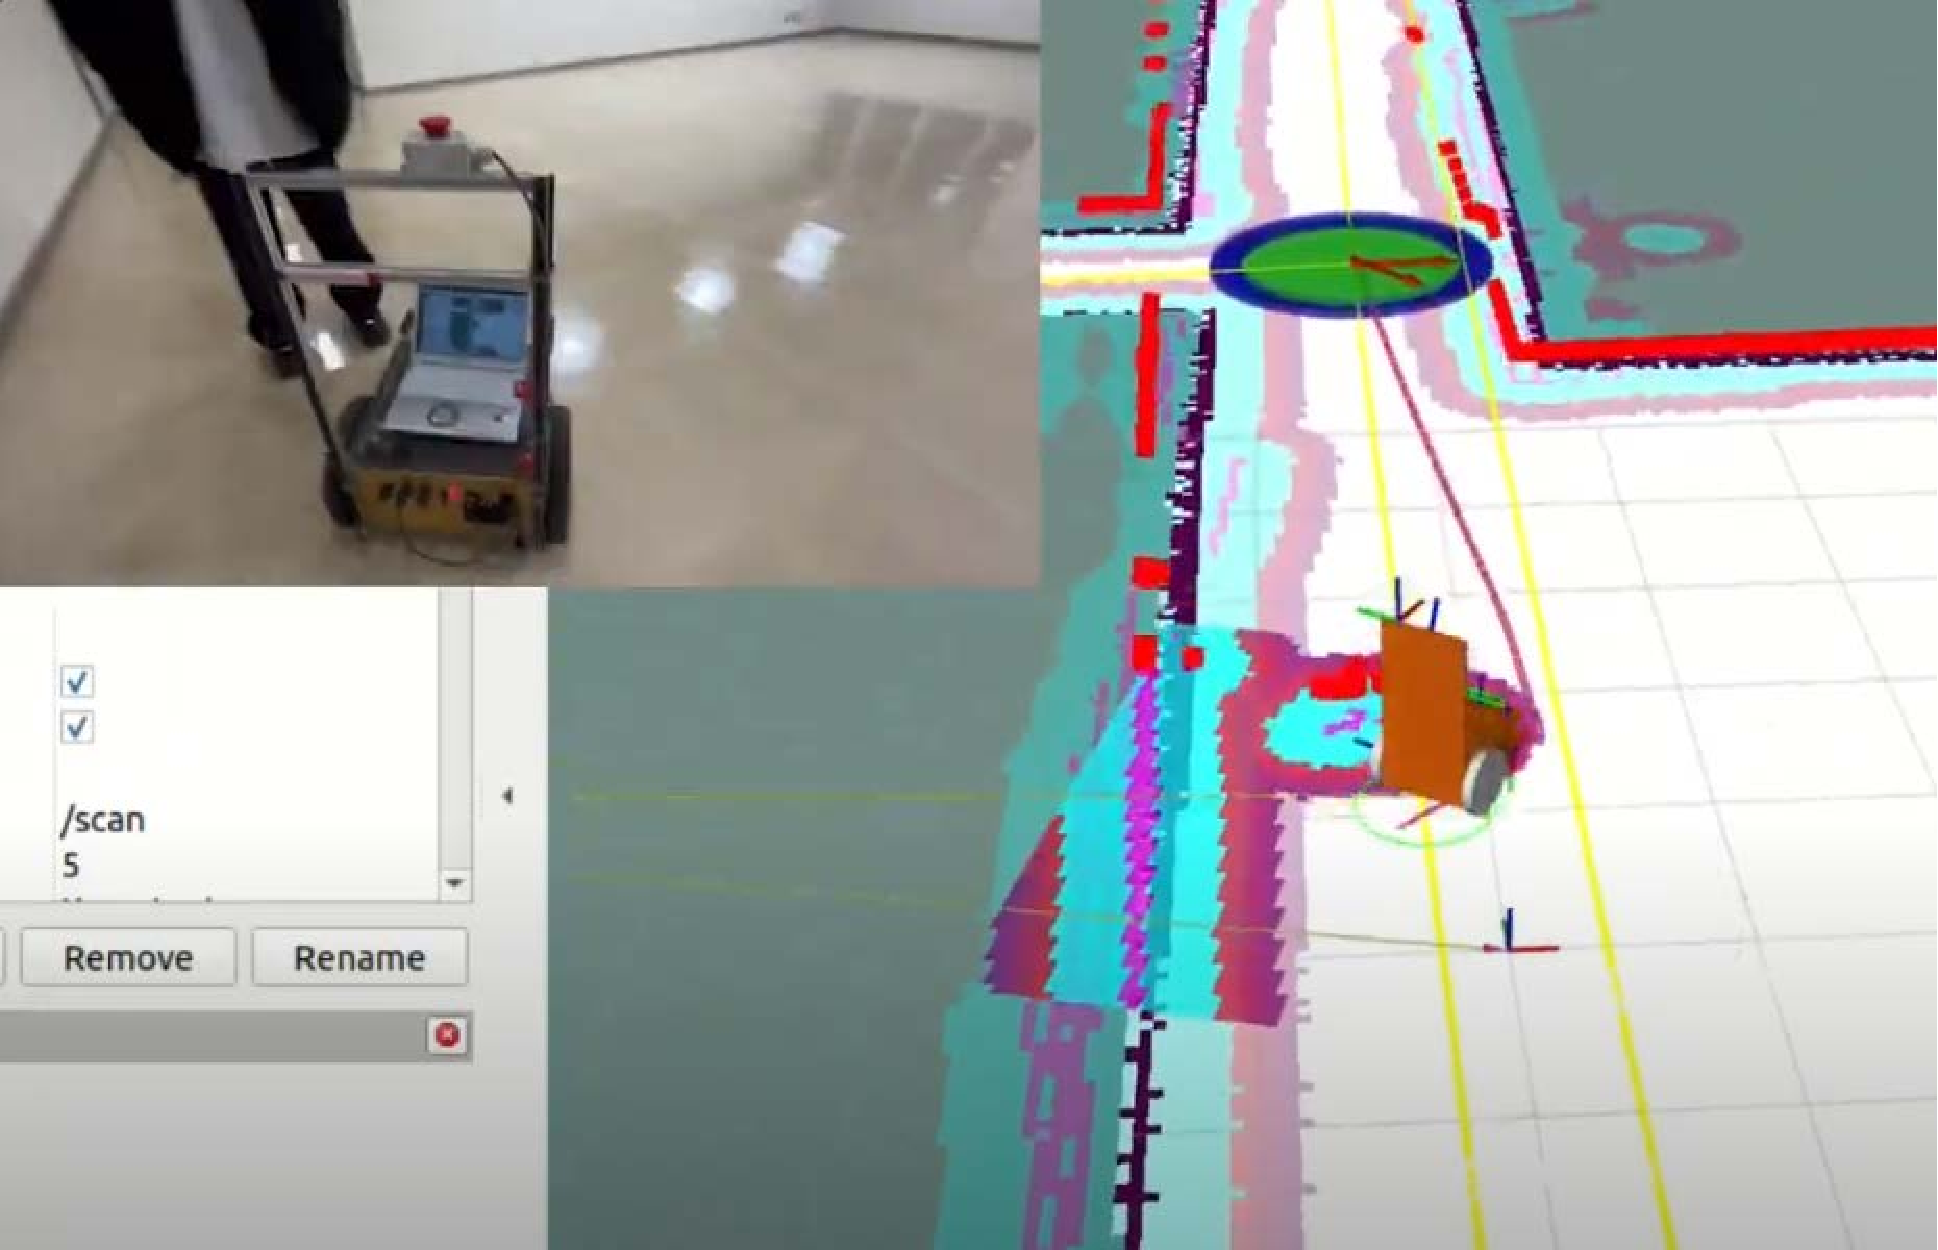
\includegraphics[width=130mm]{images/pdf/other/nav.pdf}
  \caption{Navigation based on metric map}
  \label{fig:nav}
\end{figure}